\chapter{The hardware}
\label{atomics}

\begin{figure*}[!t]
	\centering
	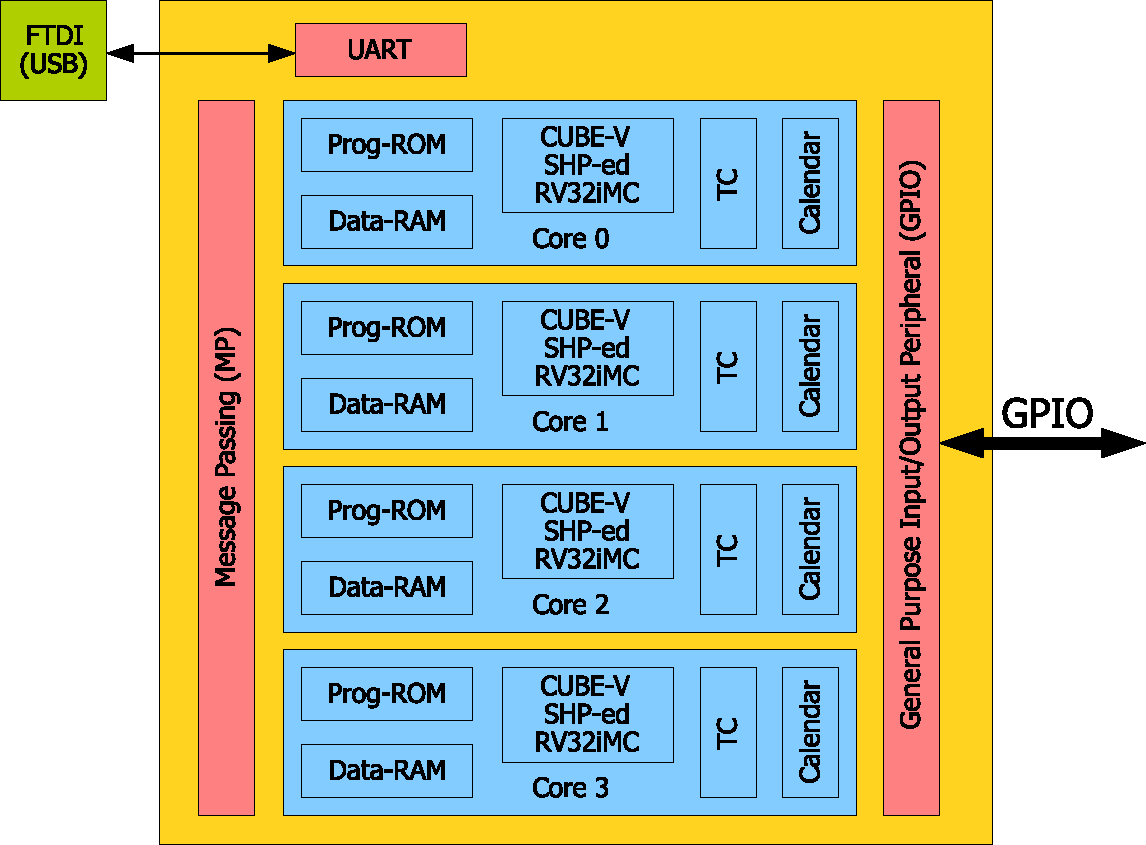
\includegraphics[width=6in]{figs/overview}
	\caption{Overview of the FPGA design.}
	\label{overview}
\end{figure*}

The hardware consists of 4 cores and some supporting peripherals (see Figure \ref{overview}). 

Each core has one CUBE-V processor, program and data memories as well one thread controller (TC) and one calendar (CA). 

The peripherals are one UART (which is connected to the FTDI chip on the ARTY board), one message passing (MP) block and a GPIO block. The cores can communicate with each other using message passing. They have equal rights to access the GPIO. Only core 0 can communicate with the UART. The UART (USB interface) is also used to download program (or data) and to readback the data-RAM of all cores.


\begin{figure*}[!t]
	\centering
	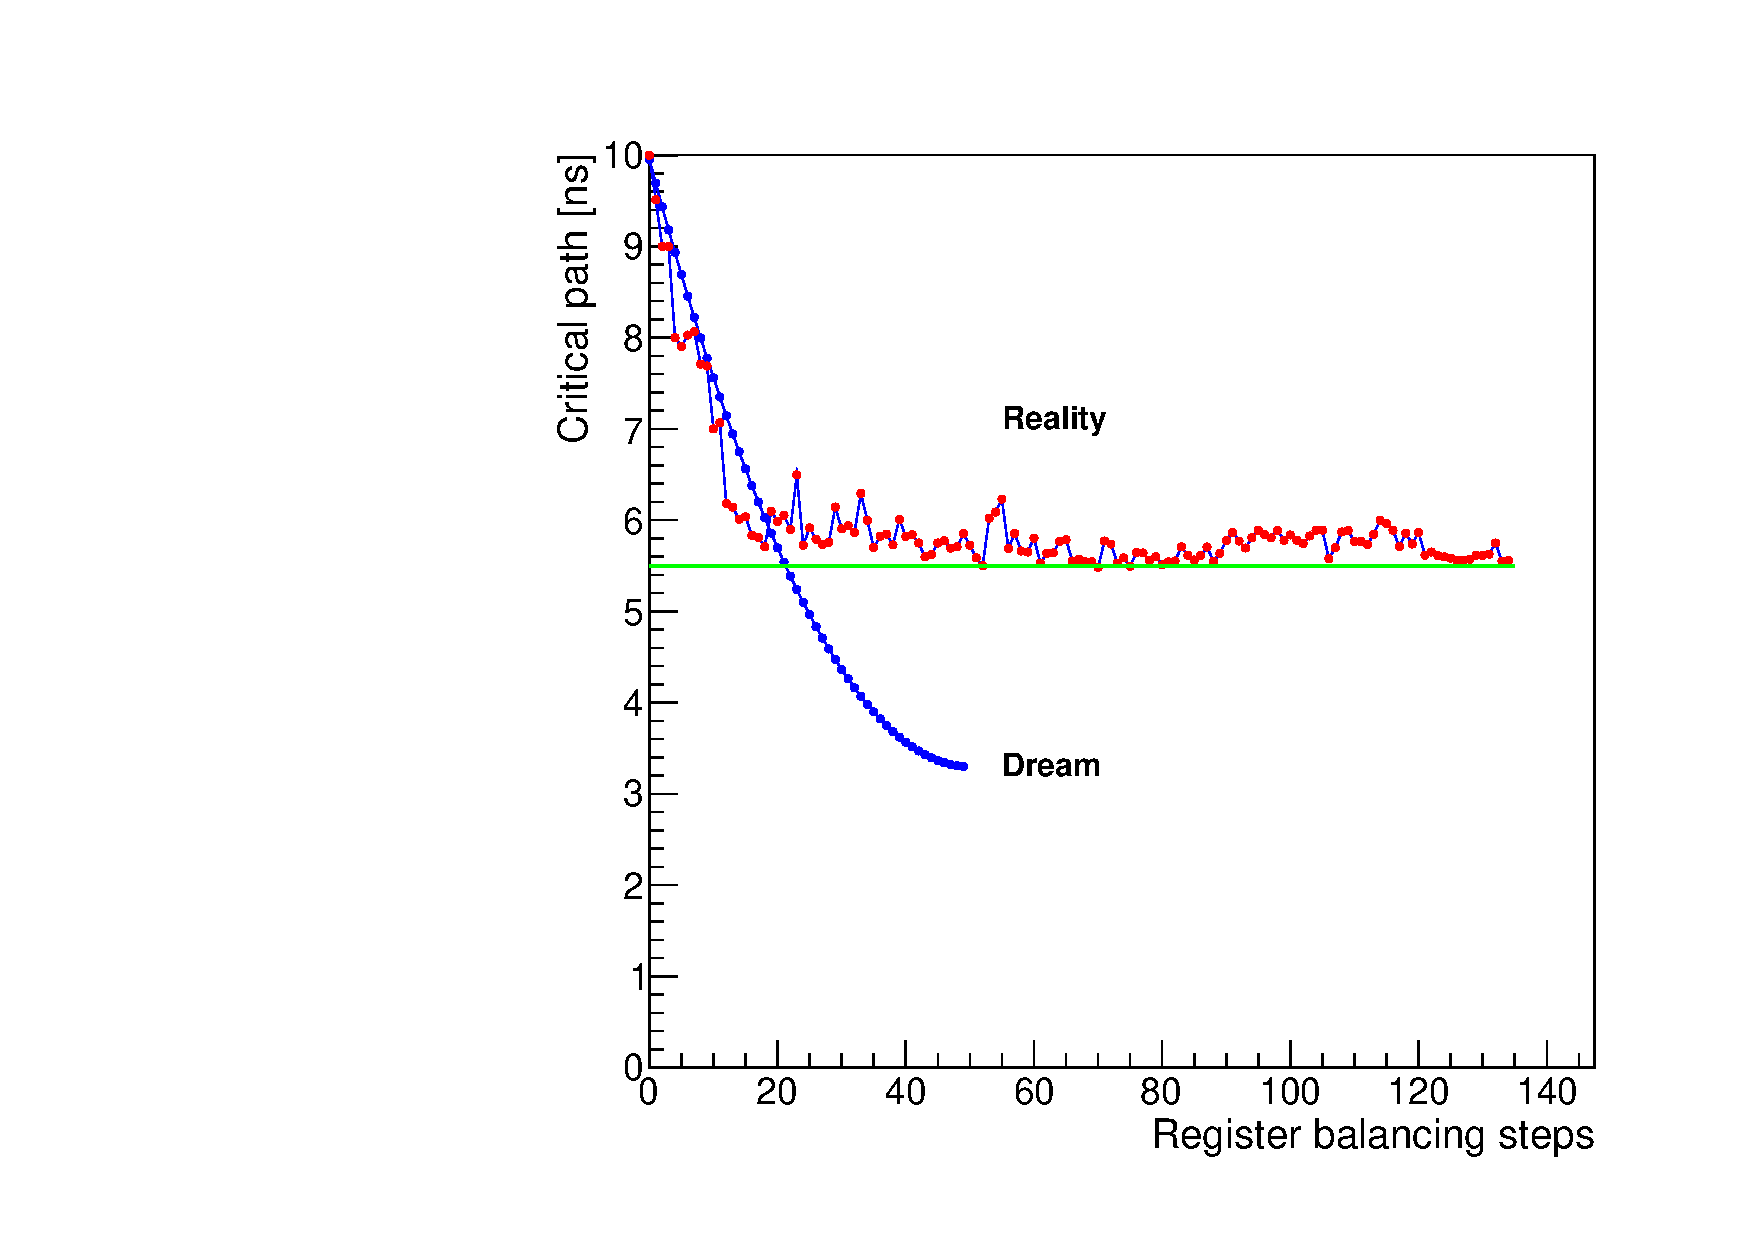
\includegraphics[width=6in]{figs/register_balancing}
	\caption{Register balancing steps of SHP-ed RV32iMC on Artix-7.}
	\label{balancing}
\end{figure*}

\section{Clocking and performance}

The system runs at 180 MHz. A micro-cycle takes therefore 5.55 nsec, a macro-cycle a minimum of 22.22 nsec. A thread runs at 45 MHz when less or equal than 4 threads are active at a time. When all 16 threads of a core are active, all threads run at 11.25 MHz.

\vspace{1in}
For performance evaluation is based on the famous CHStone testcases \url{http:/www.ertl.jp/chstone/}. They are used in the processor and the high level synthesis (HLS) domain in many papers. I explicitly use the GSM, ASM, Motion, ADCPM, SHA and Blowfish testcase. When running these testcases stand-alone an IPC (instructions per cycle) of 0,86 is reached, which results in 155 MIPS (million instructions per second) per core. When projected on the complete system 620 MIPS are reached.

Figure \ref{balancing} shows the performance increase during register balancing. Register balancing is the process to move the additional registers (which are added to the design during the C-Slow Retiming step) through the design to achieve the highest possible performance. The goal based on the early estimations was to reach 3.3 nsec, which would have resulted in a 300MHz micro-cycle performance, 1.2 GHz “clock performance” overall and 1.05 GIPS (Giga instructions per cycle). Unfortunately, as Figure \ref{balancing} shows, I run into a virtual place and route barrier at 5.55 nsec. I was way more successful with this method when doing it on a Thumb-2 based design with a "longer" critical starting path.



\section{Reset}

After power up or when the external reset button on the ARTY board was active, the complete design is in reset  mode. Each core has its own reset flag. These reset flags can only be deactivated by the UART/USB interface, by writing the right value to the right address. The same interface can also activate the individual flags again. Please refer to Section ''Download bit and hex files to the ARTY board''.

Once the reset of a core is disabled then the initial thread of that core becomes active. This active thread after reset starts at address 0x0000. 


\section{RISC-V, RV32iMC, “CUBE-V-RV32iMC-P3C4D16”}

The project uses a RV32iMC implementation of the RISC-V. It is called ''CUBE-V''. It does not support the FENCE, ECALL and EBREAK instructions and it is therefore not fully RV32I compatible, which I indicate by using the lower case ''i'' in RV32iMC.

CUBE-V also does not support the control and status registers ''CSR''.

A CUBE-V has 3 pipeline stages (''P3''). 

The complete design runs at 180MHz.  This clock generates what we call a micro-cycle. 

We applied C-Slow-Retiming generating 4 copies of each CUBE-V core (''C4''). It therefore takes 4 micro-cycles to finish one functional cycle, or in other words one macro-cycle is equal to 4 micro-cycles. 

We then apply the final SHP-step, using a memory depth of 16 lines (''D16'') to be able to run up to 16 threads at the same time on each core. We define, that a program (also called a thread) is executed at macro-cycle speed.

Unlike other high speed RV32 implementations, almost all instructions are executed in one macro-cycle. The exceptions are:

DIV[U] and REM[U]: 33 macro-cycles (might be optimized)\\
MULH[[S]U] 64-bit: 2 macro-cycles\\
Data memory read: 2  macro-cycles\\
GPIO register read: 8 micro-cycles\\

\begin{figure*}[!t]
	\centering
	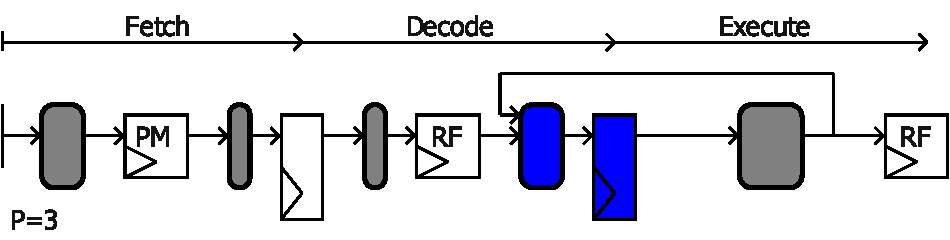
\includegraphics[width=6in]{figs/writethrough}
	\caption{Pipeline stages and register file write-through short cut.}
	\label{writethrough}
\end{figure*}

A register file (RF) write-through policy is implemented. This means, when a register dependency is detected, then the register value is not only written into the RF, but also at the output of the RF, so that the data can be used already in the next cycle (Figure \ref{writethrough}). There are only a few exceptions to this rule.

The number of active threads can be changed dynamically. When less or equal 4 threads are executed, then each thread runs at a macro-cycle speed of (180MHz / 4 =) 45 MHz. When more than 4 threads are active, let's say n, then each thread runs at a macro-cycle speed of 180MHz / n. 



\section{On-chip memory}

Each RV32iMC core has it own 6144x32 bits (24 KB) of program memory and 1024x32 bits (4 KB) of data memory. This can certainly be a limitation. In a next version, the number of cores can be reduced, which leaves more memory to individual cores. The external memory DDR3L on the ATRY board might be connected in one of the next versions at the cost of at least one CUBE-V.

It should be mentioned, that each thread on a core shares the same memory. So a peripheral driver code is shared among all virtual peripherals for instance.  It is important to know that each thread also shares the same stack, which can be problematic, unless the stack pointer is taken care of.


\section{Thread controller (TC)}

Each core is supported by an individual thread controller (TC). A thread can be initialized by one of the sources listed in Table \ref{prio}, which also lists the overall execution priority. 

\begin{table}[h]
	{
		\begin{small}
			\begin{center}
				\begin{tabular}{c c}
					\hline
					\multicolumn{1}{|c|}{Source} &
					\multicolumn{1}{|c|}{Priority} \\
					\hline
					\multicolumn{1}{|c|}{Write to TC\_START, TC\_SAK} &
					\multicolumn{1}{|c|}{6} \\
					\hline
					\multicolumn{1}{|c|}{Calendar} &
					\multicolumn{1}{|c|}{5} \\
					\hline
					\multicolumn{1}{|c|}{GPIO} &
					\multicolumn{1}{|c|}{4} \\
					\hline
					\multicolumn{1}{|c|}{MP} &
					\multicolumn{1}{|c|}{3} \\
					\hline
					\multicolumn{1}{|c|}{UART RX} &
					\multicolumn{1}{|c|}{2} \\
					\hline
					\multicolumn{1}{|c|}{UART TX} &
					\multicolumn{1}{|c|}{1} \\
					\hline
					\multicolumn{1}{|c|}{Thread FIFO} &
					\multicolumn{1}{|c|}{0} \\
					\hline
				\end{tabular}
			\end{center}
		\end{small}
	}
	\caption{Thread initialization sources and thread priorities.}
	\label{prio}
\end{table}

A thread is started by writing its program start address to the \textbf{TC\_START} or \textbf{TC\_SAK} (TC start and kill) register. An individual thread ID is automatically applied to a thread when started. So far the thread ID wasn't relevant for programming and up to now it cannot be read. There is no exception called when more than 16 threads are initialized. Instead incoming events are stalled, until they can be served. Nevertheless, still a deadlock situation can occur when the system is poorly programmed.

\begin{figure}[!t]
	\centering
	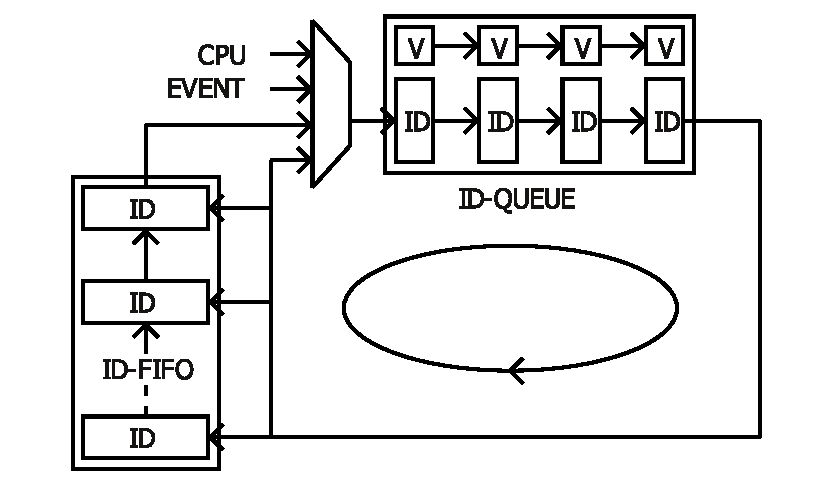
\includegraphics[width=4in]{figs/tc_fifo}
	\caption{Abstract view of the thread controller mechanism.}
	\label{fifo}
\end{figure}


Figure \ref{fifo} shows that once a thread (with a certain thread identification number ''ID'' and valid flag ''V'') leaves the hyper-pipelined execution mechanism, it is reinserted into the execution mechanism again by default. When another thread needs to be initialized at that very cycle (by the CPU or a peripheral event) or the so-called ID-FIFO contains thread(s) waiting to be executed, then the thread itself is ''parked'' in the ID-FIFO instead. In the case when multiple threads a waiting to be executed, the thread which has the highest priority listed in Table \ref{prio} is executed. The priority scheme is fixed and cannot be modified (as of now). Events are stalled when threads with higher priorities are served instead.

A thread kills itself by writing to its \textbf{TC\_SAK} register or by writing (any value) to its \textbf{TC\_KILL}  register (Table \ref{tc}).

\begin{table}[h]
	{
		\begin{small}
			\begin{center}
	\begin{tabular}{c c c c c}
		& & &
		\instbitrange{31}{14} &
		\instbitrange{13}{0} \\
		\hline
		\multicolumn{1}{|c|}{\textbf{TC\_START}} &
		\multicolumn{1}{|c|}{0x80000000} &
		\multicolumn{1}{|c|}{w} &
		\multicolumn{1}{|c|}{don't care} &
		\multicolumn{1}{|c|}{thread start address [14:1]} \\
		\hline
		\multicolumn{1}{|c|}{\textbf{TC\_KILL}} &
		\multicolumn{1}{|c|}{0x80000004} &
		\multicolumn{1}{|c|}{w} &
		\multicolumn{1}{|c|}{don't care} &
		\multicolumn{1}{|c|}{don't care} \\
		\hline
		\multicolumn{1}{|c|}{\textbf{TC\_SAK}} &
		\multicolumn{1}{|c|}{0x80000008} &
		\multicolumn{1}{|c|}{w} &
		\multicolumn{1}{|c|}{don't care} &
		\multicolumn{1}{|c|}{thread start address [14:1]} \\
		\hline
		& & &
		18 & 14 \\
	\end{tabular}
			\end{center}
		\end{small}
	}
	\caption{Registers: \textbf{TC\_START}, \textbf{TC\_KILL}, \textbf{TC\_SAK}.}
	\label{tc}
\end{table}


Threads can be initialized by writing into the \textbf{TC\_START} or \textbf{TC\_SAK} register the new thread's start address (Table \ref{tc}). When a new thread is initialize by hardware this start address must be programmed ahead of time into the relevant peripheral's register. An example procedure is described in more detail in the ''Event handling and virtual peripherals'' Chapter.


\section{Calendar (CA)}

Each SHP-ed RV32iMC core is supported by an individual calendar (CA). The CA is equivalent to a basic timer but can hold up to 240 entries. It can be written just like any other peripheral and stores a timely ordered list of future events. The CA can access GPIO registers or it can initiate a new thread once the time counter reaches the timestamp of the first event in the list.

A CA entry is a combination of a calendar command \textbf{CA\_COM} and an event time \textbf{CA\_ET}. The command register \textbf{CA\_COM} must be programmed first. It is thread specific, which means that each thread has its own \textbf{CA\_COM} register. It cannot be overwritten by another thread. 

\begin{table}[h]
	{
		\begin{center}
			\begin{tabular}{c c c c c c c c}
				\\
				& & & &
				\instbitrange{31}{29} &
				\instbitrange{28}{12} &
				\instbitrange{11}{8} &
				\instbitrange{7}{0} \\
				\hline
				\multicolumn{1}{|c|}{\textbf{CA\_COM}} &
				\multicolumn{1}{c|}{0x80001000} &
				\multicolumn{1}{|c|}{w} &
				\multicolumn{1}{|c|}{command} &
				\multicolumn{1}{c|}{code} &
				\multicolumn{1}{c|}{not used} &
				\multicolumn{1}{c|}{port} &
				\multicolumn{1}{c|}{pin} \\
				\hline
				& & & & 3 & 17 & 4 & 8 \\
				& & & clear bank & 000 & & port number & pin[7:0] \\
				& & & set bank & 001 & & port number & pin[7:0] \\
				& & & clear output & 010 & & port number & pin[7:0] \\
				& & & set output  & 011 & & port number & pin[7:0] \\
			\end{tabular}
		\end{center}
	}
	\caption{Register: CA Commands (\textbf{CA\_COM}).}
	\label{ca_com_reg}
\end{table}


\begin{table}[h]
	{
		\begin{center}
			\begin{tabular}{c c c c c c c}
				\\
				&& & &
				\instbitrange{31}{30} &
				\instbitrange{29}{14} &
				\instbitrange{13}{0} \\
				\hline
				\multicolumn{1}{|c|}{\textbf{CA\_ET}} &
				\multicolumn{1}{c|}{0x80001004} &
				\multicolumn{1}{|c|}{w} &
				\multicolumn{1}{|c|}{command} &
				\multicolumn{1}{c|}{code} &
				%\multicolumn{1}{c|}{not used} &
				\multicolumn{1}{c|}{a0\_value [15:0]} &
				\multicolumn{1}{c|}{thread start address [14:1]} \\
				\hline
				& & & & 2 & 16 & 14 \\
				& & & no a0 load & 10 &  & start address \\
				& & & with a0 load & 11 & a0\_value & start address \\
			\end{tabular}
		\end{center}
	}
	\caption{Register: CA Event Time (\textbf{CA\_ET}).}
	\label{ca_et}
\end{table}

Writing to the \textbf{CA\_ET} starts a mechanism, which picks up the thread specific \textbf{CA\_COM} value, combines it with the \textbf{CA\_ET} value and inserts this new entry in a timely ordered linked list. If a second \textbf{CA\_ET} write follows, the last \textbf{CA\_COM} entry of that thread is used again. Writing to the \textbf{CA\_ET} takes one cycle for the writing thread, but stalls any other thread which tries to write to the CA after that, until the event is inserted in the timely ordered linked list.

The user can read the value of the freely running 23-bit wide current timer register \textbf{CA\_CT} at any given time (see Table \ref{ca_ct}). A cycle takes (1 / 180 MHz =) 5.55nsec. The timer starts at 0 again after an overflow. In order to handle the overflow problematic, the following constraint is defined. The user may only program an event which is 2\textsuperscript{22-1} ( = 1f.ffffh = 2.097.151d) cycles ahead of the current time. At the same time, the user does not need to take care of the overflow and can write a low 23-bit wide value, which will be considered as an event after the next overflow. This period is equivalent to 11.6 msec when running at a frequency of 180 MHz. Longer periods must be handled by software counters and multiple events. 

The associated command is issued, once the \textbf{CA\_CT} timer matches any of the programmed event time. This command execution takes 5 cycles and is executed immediately. When multiple events should occur at the same time, they are handled sequentially with 8 cycle delay time. It is therefore recommended to assign an offset to individual event groups, in order to reduce this “late” command execution, in case a very precise timing is required.

\begin{table}[h]
	{
		\begin{center}
			\begin{tabular}{c c c c c}
				\\
				& & &
				\instbitrange{31}{24} &
				\instbitrange{22}{0} \\
				\hline
				\multicolumn{1}{|c|}{\textbf{CA\_CT}} &
				\multicolumn{1}{c|}{0x80001008} &
				\multicolumn{1}{|c|}{r} &
				\multicolumn{1}{c|}{0} &
				\multicolumn{1}{c|}{current time} \\
				\hline
				& & & 9 & 23 \\
			\end{tabular}
		\end{center}
	}
	\caption{Register: CA Current Time (\textbf{CA\_CT}).}
	\label{ca_ct}
\end{table}

Another delay of an event execution can occur, when an entry is inserted into the linked list and the algorithm just checks the very first entry of this list. The command execution is disabled during these 7 cycles. For the remaining time of the entry insertion period, one match can be handled.

The CA looks back 2\textsuperscript{12-1} ( = fffh = 4095d ) cycles to catch up with missed matches.

A command can access GPIO registers or can initiate a thread. 

A GPIO command can clear and set individual GPIO port directions and output values (see Table \ref{ca_com_reg}).

A CA can also be programmed to directly start a thread at a programmable thread start address. It can be defined, whether a data value of 16 bits is copied over into the register file at address 10d (register name a0) or not (see Table \ref{ca_et}). %A programming example can be found in Section N.

\section{Message Passing (MP)}

The message passing feature is implemented as a simple 32 bit wide data transfer from a transmitting core tx to a receiving core rx. All permutations with tx = {0, 1, 2, 3} and rx = {0, 1, 2, 3} are valid except for data transfer within a single core. The relevant registers are listed in Table \ref{mp_registers_1} and \ref{mp_registers_2}.

The MP peripheral can transfer data in two modes. Either the receiving data is read when valid, or the tranmitting core initiates a thread in the receiving core.

For a data transfer from tx to rx, the transmitting core tx writes the 32-bit wide data to its “message passing out-going” register \textbf{MP\_OUT\_[rx]}. This data is then “transferred” to the “message passing in-coming” register of the receiving core \textbf{MP\_IN\_[tx]}. The transmitting core tx stalls until the message is read from the message receiving core.

The MP peripheral can be programmed to initiate a thread at the receiving core, once a new message is valid. To enable this mechanism, bit 14 must be set in the \textbf{MP\_COM\_[rx]} register, and the thread start address must be programmed as well (see Table \ref{mp_registers_2}). Still, the transmitting core stalls until the receiving register \textbf{MP\_IN\_[rx]} is read. 

\begin{table}[h]
	{
		\begin{center}
			\begin{tabular}{c c c c}
						& & &
						\instbitrange{31}{0} \\ \hline
		\multicolumn{1}{|c|}{\textbf{MP\_OUT\_0}}	& \multicolumn{1}{c|}{0x80040000} & \multicolumn{1}{c|}{w} & \multicolumn{1}{c|}{send data} \\ \hline
		\multicolumn{1}{|c|}{\textbf{MP\_OUT\_1}}	& \multicolumn{1}{c|}{0x80040004} & \multicolumn{1}{c|}{w} & \multicolumn{1}{c|}{send data} \\	\hline
		\multicolumn{1}{|c|}{\textbf{MP\_OUT\_2}}	& \multicolumn{1}{c|}{0x80040008} & \multicolumn{1}{c|}{w} & \multicolumn{1}{c|}{send data} \\	\hline
		\multicolumn{1}{|c|}{\textbf{MP\_OUT\_3}}	& \multicolumn{1}{c|}{0x8004000c} & \multicolumn{1}{c|}{w} & \multicolumn{1}{c|}{send data} \\	\hline
		\multicolumn{1}{|c|}{\textbf{MP\_IN\_0}}	& \multicolumn{1}{c|}{0x80040010} & \multicolumn{1}{c|}{r} & \multicolumn{1}{c|}{receive data} \\ \hline
		\multicolumn{1}{|c|}{\textbf{MP\_IN\_1}}	& \multicolumn{1}{c|}{0x80040014} & \multicolumn{1}{c|}{r} & \multicolumn{1}{c|}{receive data} \\ \hline
		\multicolumn{1}{|c|}{\textbf{MP\_IN\_2}}	& \multicolumn{1}{c|}{0x80040018} & \multicolumn{1}{c|}{r} & \multicolumn{1}{c|}{receive data} \\ \hline
		\multicolumn{1}{|c|}{\textbf{MP\_IN\_3}}	& \multicolumn{1}{c|}{0x8004001c} & \multicolumn{1}{c|}{r} & \multicolumn{1}{c|}{receive data} \\ \hline
	\end{tabular}
\end{center}
	}
	\caption{Register: Message passing out and in (\textbf{MP\_OUT\_N, MP\_IN\_N}).}
	\label{mp_registers_1}
\end{table}


\begin{table}[h]
	{
\begin{center}
	\begin{tabular}{c c c c c}
		& & &
		\instbitrange{14}{14} &
		\instbitrange{13}{0} \\ \hline
		\multicolumn{1}{|c|}{\textbf{MP\_COM\_0}} & \multicolumn{1}{c|}{0x80040020} & \multicolumn{1}{c|}{w} & \multicolumn{1}{c|}{thread enable bit} & \multicolumn{1}{c|}{thread start address [14:1]}\\ \hline
		\multicolumn{1}{|c|}{\textbf{MP\_COM\_1}} & \multicolumn{1}{c|}{0x80040024} & \multicolumn{1}{c|}{w} & \multicolumn{1}{c|}{thread enable bit} & \multicolumn{1}{c|}{thread start address [14:1]}\\ \hline
		\multicolumn{1}{|c|}{\textbf{MP\_COM\_2}} & \multicolumn{1}{c|}{0x80040028} & \multicolumn{1}{c|}{w} & \multicolumn{1}{c|}{thread enable bit} & \multicolumn{1}{c|}{thread start address [14:1]}\\ \hline
		\multicolumn{1}{|c|}{\textbf{MP\_COM\_3}} & \multicolumn{1}{c|}{0x8004002c} & \multicolumn{1}{c|}{w} & \multicolumn{1}{c|}{thread enable bit} & \multicolumn{1}{c|}{thread start address [14:1]}\\ \hline
	\end{tabular}
\end{center}
	}
	\caption{Register: Message passing communication control (\textbf{MP\_COM\_N}).}
	\label{mp_registers_2}
\end{table}


\section{GPIO}

The GPIO peripheral is accessible by all cores. It supports 14 banks with 8 pins each and therefore 112 pins. Its register set is optimized towards the connector bundles (8-bits) of the ARTY board. The direction can be set (output) or cleared (input) for each pin using the \textbf{GPIO\_N\_DIR\_SET} or the \textbf{GPIO\_N\_DIR\_CLR} register respectively (see Table \ref{gpio_bank}). N stands for the bank number. The setting of the bit in the \textbf{GPIO\_N\_OUT\_SET} (\textbf{GPIO\_N\_OUT\_CLR}) register makes an output pin switch to 3.3V (ground). 

\begin{table}[h]
	{
		\begin{small}
			\begin{center}
				\begin{tabular}{c c c c c}
					& offset  & &
					\instbitrange{31}{8} &
					\instbitrange{7}{0} \\
					\hline
					\multicolumn{1}{|c|}{\textbf{GPIO\_N\_DIR\_CLR}} &
					\multicolumn{1}{|c|}{0x0000} &
					\multicolumn{1}{|c|}{w} &
					\multicolumn{1}{|c|}{don't care} &
					\multicolumn{1}{|c|}{pin[7:0]} \\
					\hline
					\multicolumn{1}{|c|}{\textbf{GPIO\_N\_DIR\_SET}} &
					\multicolumn{1}{|c|}{0x0004} &
					\multicolumn{1}{|c|}{w} &
					\multicolumn{1}{|c|}{don't care} &
					\multicolumn{1}{|c|}{pin[7:0]} \\
					\hline
					\multicolumn{1}{|c|}{\textbf{GPIO\_N\_OUT\_CLR}} &
					\multicolumn{1}{|c|}{0x0010} &
					\multicolumn{1}{|c|}{w} &
					\multicolumn{1}{|c|}{don't care} &
					\multicolumn{1}{|c|}{pin[7:0]} \\
					\hline
					\multicolumn{1}{|c|}{\textbf{GPIO\_N\_OUT\_SET}} &
					\multicolumn{1}{|c|}{0x0014} &
					\multicolumn{1}{|c|}{w} &
					\multicolumn{1}{|c|}{don't care} &
					\multicolumn{1}{|c|}{pin[7:0]} \\
					\hline
					\multicolumn{1}{|c|}{\textbf{GPIO\_N\_IN}} &
					\multicolumn{1}{|c|}{0x0020} &
					\multicolumn{1}{|c|}{r} &
					\multicolumn{1}{|c|}{0} &
					\multicolumn{1}{|c|}{pin[7:0]} \\
					\hline
					\multicolumn{1}{|c|}{\textbf{GPIO\_N\_LVL0}} &
					\multicolumn{1}{|c|}{0x0030} &
					\multicolumn{1}{|c|}{w} &
					\multicolumn{1}{|c|}{don't care} &
					\multicolumn{1}{|c|}{pin[7:0]} \\
					\hline
					\multicolumn{1}{|c|}{\textbf{GPIO\_N\_LVL1}} &
					\multicolumn{1}{|c|}{0x0034} &
					\multicolumn{1}{|c|}{w} &
					\multicolumn{1}{|c|}{don't care} &
					\multicolumn{1}{|c|}{pin[7:0]} \\
					\hline
					\multicolumn{1}{|c|}{\textbf{GPIO\_N\_CAP}} &
					\multicolumn{1}{|c|}{0x0040} &
					\multicolumn{1}{|c|}{w} &
					\multicolumn{1}{|c|}{don't care} &
					\multicolumn{1}{|c|}{pin[7:0]} \\
					\hline
					& & &
					24 & 8 \\
				\end{tabular}
			\end{center}
		\end{small}
	}
	\caption{Registers: \textbf{GPIO\_N\_DIR\_CLR, GPIO\_N\_DIR\_SET, GPIO\_N\_OUT\_CLR, GPIO\_N\_OUT\_SET, GPIO\_N\_IN, GPIO\_N\_LVL0, GPIO\_N\_LVL1, GPIO\_N\_CAP}}
	\label{gpio_bank}
\end{table}

The value of each GPIO pin can be read by accessing the \textbf{GPIO\_N\_IN} register. The input signal passes always through a filter first. It uses a 3 bit-wide shift register running at 180MHz. A majority decoder extracts the actual (filtered) signal value.

Each GPIO pin of the first 9 banks can be programmed to be level (and therefore edge) sensitive. Setting a bit in the \textbf{GPIO\_N\_LVL0} (\textbf{GPIO\_N\_LVL1}) registers programs the input logic of the relevant bit to be level sensitive to low (high). The level sensitive logic uses the filtered input signal only.

Once the relevant signal matches the programmed input level (zero or one) the GPIO starts an internal event handling mechanism. When the level matches the programmed input level during programming already, then this event handling mechanism is started immediately. If not, it starts one cycle after the filtered input signal reaches the programmed level. It can be argued, that this mechanism is therefore (also) edge sensitive.

One task of the event handling mechanism is to capture the filtered input signal of the neighboring pin with the next higher index of the same bank. This value is then stored in the readable \textbf{GPIO\_N\_CAP} register at the bit location of the neighboring pin with the next higher index. If the level sensitive pin is at bit 7 of the bank, then the neighboring pin is bit 0 of the same bank.

Another task of the event handling mechanism is to start a thread at a predefined program address. A round robin arbiter mechanism takes care, that all events are propagated with the same priority and that no event is missed due to multiple consecutive events of some other pin(s).

8 cycles after the relevant filtered signal equals the defined level, the GPIO peripheral requests from the TC to initiate a thread at a programmable start address. (In other terms, 15 cycles (83 nsec) from an input edge to the first program fetch of the start address, which is very fast, considering the fact, that a filter and an arbiter is involved). Each core can program its core specific thread start address into the core specific \textbf{GPIO\_EVENT\_ADD} register (see Ttable \ref{gpio_event}). The event is propagated to only one single core. The core is selected, which was the last one to program the pin specific \textbf{GPIO\_N\_LVL0} or \textbf{GPIO\_N\_LVL1} registers. Also, all events for one core end up at the same thread starting address. 

%A programming example can be found in Section N.

\begin{table}[h]
	{
		\begin{small}
			\begin{center}
				\begin{tabular}{c c c c c}
					& & &
					\instbitrange{31}{14} &
					\instbitrange{13}{0} \\
					\hline
					\multicolumn{1}{|c|}{\textbf{GPIO\_EVENT\_ADD}} &
					\multicolumn{1}{|c|}{0x80031000} &
					\multicolumn{1}{|c|}{w} &
					\multicolumn{1}{|c|}{don't care} &
					\multicolumn{1}{|c|}{thread start address [14:1]} \\
					\hline
					& & &
					18 & 14 \\
				\end{tabular}
			\end{center}
		\end{small}
	}
	\caption{Register: \textbf{GPIO\_EVENT\_ADD}}
	\label{gpio_event}
\end{table}

The program needs to know, which input pin started the particular event. For that, the global pin index is propagated into the link register 10d (a0) of the core register file. The global pin index is the result of the bank number multiplier by 8, plus the pin location within the bank. In other words, it is a unique pin number.

Once an event has been handled and a thread is initialized, the pin specific level sensing mechanism needs to be reprogrammed. The \textbf{GPIO\_EVENT\_ADD} does not need to be reprogrammed.

Due to area limitations of the FPGA, the GPIOs supporting incoming event propagation is scaled down to 72 pins (first 9 banks). The upper banks are connected to LEDs and switches anyway.

The base address of the GPIO block is 0x80031000.

The address step to the next bank addressing is 0x100.

For more information please see the ''Register map'' Chapter.

\section{UART}

The implemented UART is used for communication with the external FTDI USB chip at a fixed baudrate of 5 MBaud. The system can therefore communicate with a PC (for example) via USB. The UART peripheral communicates internally only with core 0. Nevertheless, program and data memories of all cores can be written and data memories of all cores can be read via this PC-link as well. Please see Chapter ''Download bit and hex files to the ARTY board'' for more information.

The UART uses 3 registers for controlling the sending mechanism (\textbf{UART\_SEND, UART\_SEND\_STAT, UART\_TX\_COM}) and 3 registers for the receiving part (\textbf{UART\_REC, UART\_REC\_STAT, UART\_RX\_COM}). They are listed in Table \ref{uart_trx}, \ref{uart_trx_stat} and \ref{uart_trx_com}.

Both directions can be executed in normal or advanced mode.

When a byte should be send via the UART to the FTDI chip in normal mode, then the data must be written into the \textbf{UART\_SEND} register. When the UART is still busy sending the last byte, then the thread trying to write to the \textbf{UART\_SEND} register is stalled until the sending of the last byte has finished. This allows a simple programming of a thread which serves as DMA engine. In case the stalling should be reduced, the send\_busy flag in the \textbf{UART\_SEND\_STAT} register can be polled to check whether the sending block is still active.

The UART can be programmed to initiate a thread (advanced mode), once the sending of the data has finished. To enable this mechanism, the thread enable bit in the \textbf{UART\_TX\_COM} register must be set and the thread start address must be programmed. 

The UART can be configured using the \textbf{UART\_RX\_COM} register to handle receiving bytes in normal mode or advanced mode. In normal mode (Bit 14 in \textbf{UART\_RX\_COM} is 0) the received value can be read using the \textbf{UART\_REC} register. If the \textbf{UART\_REC} is not valid or has been read already, then the reading thread is stalled until the value is valid (again). This allows a simple programming of a thread which serves as DMA engine. In case the stalling should be reduced, the receive\_valid flag in the \textbf{UART\_REC\_STAT} register can be polled to check whether a received byte is valid.

Once the UART received a serial byte from the FTDI chip and the UART receiving part is set into advanced mode (Bit 14 in \textbf{UART\_RX\_COM} is 1), then a thread is initialized at core 0. The least significant 14 bits of the \textbf{UART\_RX\_COM} determine the start address. The received byte is valid in register a0 (register 10d) of the register file. The received value can also be read via the \textbf{UART\_REC} register in advanced mode as well.

The receive value must be read via the \textbf{UART\_REC} register or the relevant thread must be executed (received data is saved in a0), otherwise the data will be overwritten.

\begin{table}[h]
	{
		\begin{small}
			\begin{center}
				\begin{tabular}{c c c c c}
					& & &
					\instbitrange{31}{8} &
					\instbitrange{7}{0} \\
					\hline
					\multicolumn{1}{|c|}{\textbf{UART\_SEND}} &
					\multicolumn{1}{|c|}{0x80020000} &
					\multicolumn{1}{|c|}{w} &
					\multicolumn{1}{|c|}{don't care} &
					\multicolumn{1}{|c|}{send byte} \\
					\hline
					\multicolumn{1}{|c|}{\textbf{UART\_REC}} &
					\multicolumn{1}{|c|}{0x80020020} &
					\multicolumn{1}{|c|}{r} &
					\multicolumn{1}{|c|}{0} &
					\multicolumn{1}{|c|}{received byte} \\
					\hline
					& & &
					24 & 8 \\
				\end{tabular}
			\end{center}
		\end{small}
	}
	\caption{Register: \textbf{UART\_SEND}, \textbf{UART\_REC}}
	\label{uart_trx}
\end{table}

\vspace{0.3in}

\begin{table}[h]
	{
		\begin{small}
			\begin{center}
				\begin{tabular}{c c c c c}
					& & &
					\instbitrange{31}{1} &
					\instbitrange{0} {0}\\
					\hline
					\multicolumn{1}{|c|}{\textbf{UART\_SEND\_STAT}} &
					\multicolumn{1}{|c|}{0x80020004} &
					\multicolumn{1}{|c|}{w} &
					\multicolumn{1}{|c|}{don't care} &
					\multicolumn{1}{|c|}{send\_busy} \\
					\hline
					\multicolumn{1}{|c|}{\textbf{UART\_REC\_STAT}} &
					\multicolumn{1}{|c|}{0x80020024} &
					\multicolumn{1}{|c|}{r} &
					\multicolumn{1}{|c|}{0} &
					\multicolumn{1}{|c|}{receive\_valid} \\
					\hline
					& & &
					30 & 1 \\
				\end{tabular}
			\end{center}
		\end{small}
	}
	\caption{Register: \textbf{UART\_SEND\_STAT}, \textbf{UART\_REC\_STAT}}
	\label{uart_trx_stat}
\end{table}

\vspace{0.3in}

\begin{table}[h]
	{
		\begin{small}
			\begin{center}
				\begin{tabular}{c c c c c c}
					& & &
					\instbitrange{31}{15} &
					\instbitrange{14} {14}&
					\instbitrange{13}{0} \\
					\hline
					\multicolumn{1}{|c|}{\textbf{UART\_TX\_COM}} &
					\multicolumn{1}{|c|}{0x80020010} &
					\multicolumn{1}{|c|}{w} &
					\multicolumn{1}{|c|}{don't care} &
					\multicolumn{1}{|c|}{thread enable bit} &
					\multicolumn{1}{|c|}{thread start address [14:1]} \\
					\hline
					\multicolumn{1}{|c|}{\textbf{UART\_RX\_COM}} &
					\multicolumn{1}{|c|}{0x80020030} &
					\multicolumn{1}{|c|}{w} &
					\multicolumn{1}{|c|}{don't care} &
					\multicolumn{1}{|c|}{thread enable bit} &
					\multicolumn{1}{|c|}{thread start address [14:1]} \\
					\hline
					& & &
					17 & 1 & 14 \\
				\end{tabular}
			\end{center}
		\end{small}
	}
	\caption{Register: \textbf{UART\_TX\_COM}, \textbf{UART\_RX\_COM}}
	\label{uart_trx_com}
\end{table}




